\documentclass[11pt]{article}

% Change "review" to "final" to generate the final (sometimes called camera-ready) version.
% Change to "preprint" to generate a non-anonymous version with page numbers.
\usepackage[review]{acl}
\usepackage{tabularx}
% Standard package includes
\usepackage{times}
\usepackage{latexsym}
\usepackage{graphicx}
\usepackage{subfigure}
\usepackage{booktabs} % for professional tables
\usepackage{natbib}  % For \citep{} commands
\usepackage{amsmath}
\usepackage{amssymb}
\usepackage{svg}
% For proper rendering and hyphenation of words containing Latin characters (including in bib files)
\usepackage[T1]{fontenc}
% For Vietnamese characters
% \usepackage[T5]{fontenc}
% See https://www.latex-project.org/help/documentation/encguide.pdf for other character sets

% This assumes your files are encoded as UTF8
\usepackage[utf8]{inputenc}

% This is not strictly necessary, and may be commented out,
% but it will improve the layout of the manuscript,
% and will typically save some space.
\usepackage{microtype}

% This is also not strictly necessary, and may be commented out.
% However, it will improve the aesthetics of text in
% the typewriter font.
\usepackage{inconsolata}

%Including images in your LaTeX document requires adding
%additional package(s)
\usepackage{graphicx}

% If the title and author information does not fit in the area allocated, uncomment the following
%
%\setlength\titlebox{<dim>}
%
% and set <dim> to something 5cm or larger.

\title{Context-Conditioned Linear Layers for Efficient Transformers}

% Author information can be set in various styles:
% For several authors from the same institution:
% \author{Author 1 \and ... \and Author n \\
%         Address line \\ ... \\ Address line}
% if the names do not fit well on one line use
%         Author 1 \\ {\bf Author 2} \\ ... \\ {\bf Author n} \\
% For authors from different institutions:
% \author{Author 1 \\ Address line \\  ... \\ Address line
%         \And  ... \And
%         Author n \\ Address line \\ ... \\ Address line}
% To start a separate ``row'' of authors use \AND, as in
% \author{Author 1 \\ Address line \\  ... \\ Address line
%         \AND
%         Author 2 \\ Address line \\ ... \\ Address line \And
%         Author 3 \\ Address line \\ ... \\ Address line}

\author{Pearse Jim \\
  Independent Researcher / Machine Learning Collective\\
  % Affiliation / Address line 2 \\
  % Affiliation / Address line 3 \\
  \texttt{pearsejim01@gmail.com} \\\And
  % Second Author \\
  % Affiliation / Address line 1 \\
  % Affiliation / Address line 2 \\
  % Affiliation / Address line 3 \\
  % \texttt{email@domain} \\
  }

%\author{
%  \textbf{First Author\textsuperscript{1}},
%  \textbf{Second Author\textsuperscript{1,2}},
%  \textbf{Third T. Author\textsuperscript{1}},
%  \textbf{Fourth Author\textsuperscript{1}},
%\\
%  \textbf{Fifth Author\textsuperscript{1,2}},
%  \textbf{Sixth Author\textsuperscript{1}},
%  \textbf{Seventh Author\textsuperscript{1}},
%  \textbf{Eighth Author \textsuperscript{1,2,3,4}},
%\\
%  \textbf{Ninth Author\textsuperscript{1}},
%  \textbf{Tenth Author\textsuperscript{1}},
%  \textbf{Eleventh E. Author\textsuperscript{1,2,3,4,5}},
%  \textbf{Twelfth Author\textsuperscript{1}},
%\\
%  \textbf{Thirteenth Author\textsuperscript{3}},
%  \textbf{Fourteenth F. Author\textsuperscript{2,4}},
%  \textbf{Fifteenth Author\textsuperscript{1}},
%  \textbf{Sixteenth Author\textsuperscript{1}},
%\\
%  \textbf{Seventeenth S. Author\textsuperscript{4,5}},
%  \textbf{Eighteenth Author\textsuperscript{3,4}},
%  \textbf{Nineteenth N. Author\textsuperscript{2,5}},
%  \textbf{Twentieth Author\textsuperscript{1}}
%\\
%\\
%  \textsuperscript{1}Affiliation 1,
%  \textsuperscript{2}Affiliation 2,
%  \textsuperscript{3}Affiliation 3,
%  \textsuperscript{4}Affiliation 4,
%  \textsuperscript{5}Affiliation 5
%\\
%  \small{
%    \textbf{Correspondence:} \href{mailto:email@domain}{email@domain}
%  }
%}





\begin{document}
\maketitle

\begin{abstract}
Standard Transformers rely on scaling static dense layers for capacity, leading to significant memory and computational redundancy. Existing efficiency methods like Mixture-of-Experts (MoE) or static low-rank factorization introduce trade-offs in routing complexity or limited expressivity. We introduce \textbf{Context-Conditioned Linear Layers (CCL)}, a drop-in replacement for dense layers that replaces static matrices with a dynamic composition mechanism. CCL learns a compact \textit{Basis Dictionary} and a lightweight \textit{Global Context Manager}. For each token, the model dynamically modulates the basis to construct a unique, token-specific linear operator. This yields high \textit{expressed capacity}, spanning a high-dimensional subspace across the sequence, while minimizing \textit{stored capacity}. Empirical results demonstrate that CCL significantly improves perplexity–parameter trade-offs. A 10.3M parameter model achieves lower perplexity than a 70.5M dense baseline , representing a 6.8x reduction in size with superior performance, all while preserving hardware-friendly dense linear algebra.
\end{abstract}
\section{Introduction}

Linear transformations account for a substantial fraction of both parameters and computation in Transformer-based language models. As models scale, these layers increasingly dominate inference cost, motivating parameter-efficient alternatives such as low-rank factorization and mixture-of-experts (MoE) architectures. However, existing approaches expose a trade-off: static low-rank layers restrict all inputs to a fixed subspace, while MoE methods rely on sparse routing that can be memory-bound and inefficient on modern accelerators.

We address this limitation by introducing \emph{Context-Conditioned Linear Layers} (CCL), which make linear transformations explicitly dependent on input context. Instead of learning a single static weight matrix or routing tokens to experts, CCL constructs token-specific effective projections by gating a small set of shared basis components using a continuous context signal. This allows each token to induce a distinct linear transformation while reusing a compact parameterization.

Although each effective projection is low-rank, we show that the set of transformations realized across a sequence exhibits high effective rank, providing substantially greater capacity than static low-rank baselines. Importantly, CCL uses only dense matrix multiplications and elementwise operations, avoiding sparse indexing and enabling efficient execution on GPUs.

Experiments on Transformer language models demonstrate that CCL improves perplexity under matched parameter budgets and achieves favorable FLOPs–performance trade-offs. These results suggest that context-conditioned linear operators offer a simple and hardware-efficient alternative to expert-based and static low-rank designs.
\section{Related Work}

\paragraph{Efficient Transformers and Sparsity.}
The dominant approach to scaling Transformer capacity without proportional computational cost is the Mixture-of-Experts (MoE) paradigm \cite{shazeer2017outrageously, lepikhin2020gshard}. MoE models route tokens to discrete expert subnetworks, enabling massive parameter counts with constant inference FLOPs. However, MoE introduces significant challenges: routing instability, expert collapse, and hardware inefficiency due to sparse memory access patterns. Our work shares the goal of decoupling parameter count from FLOPs but diverges in mechanism. Unlike MoE, CCL uses a single dense pathway without discrete routing, preserving the hardware efficiency of dense matrix multiplications while achieving dynamic capacity via basis modulation.

\paragraph{Dynamic Weights and Hypernetworks.}
Hypernetworks \cite{ha2016hypernetworks} generate the weights of a target network based on context. While powerful, standard hypernetworks are prohibitively expensive for large language models, as generating a full $d \times d$ matrix requires $O(d^2)$ operations per token. Fast Weight Programmers \cite{schlag2021linear} and linear attention variants explore similar dynamic principles but often focus on attention mechanisms. CCL is related to rank-constrained hypernetworks. By generating only $O(d)$ gating coefficients to modulate a static basis, we achieve the expressivity of dynamic weights with negligible computational overhead.

\paragraph{Parameter-Efficient Fine-Tuning (PEFT).}
Methods like LoRA \cite{hu2021lora} use low-rank decompositions to adapt pre-trained models efficiently. However, these decompositions are static—once learned, the rank-constrained matrices are fixed for all inputs. CCL extends this principle to the dynamic regime. We employ a similar low-rank structure but modulate the subspace for every token. This allows the model to access a high-dimensional manifold of effective operators across a sequence, overcoming the expressivity bottleneck of static low-rank factorization.

\paragraph{Gated Linear Units (GLU).}
Gated Linear Units and their variants (e.g., GLU, GELU-GLU, SwiGLU) introduce multiplicative gates that modulate neuron activations within feed-forward networks \citep{dauphin2017language, shazeer2020glu}. While superficially similar, CCL operates at a different level of abstraction. GLU-style mechanisms gate individual neuron outputs after a fixed linear transformation, whereas CCL gates \emph{shared basis features} and \emph{output dimensions} to dynamically construct token-specific effective linear operators. In this sense, GLUs modulate activations under a static weight matrix, while CCL modulates the structure of the linear map itself, enabling a family of context-dependent transformations rather than a single gated projection.


\begin{figure*}[!htbp]
% \vspace{1em}
% \begin{figure}[H]
\centering
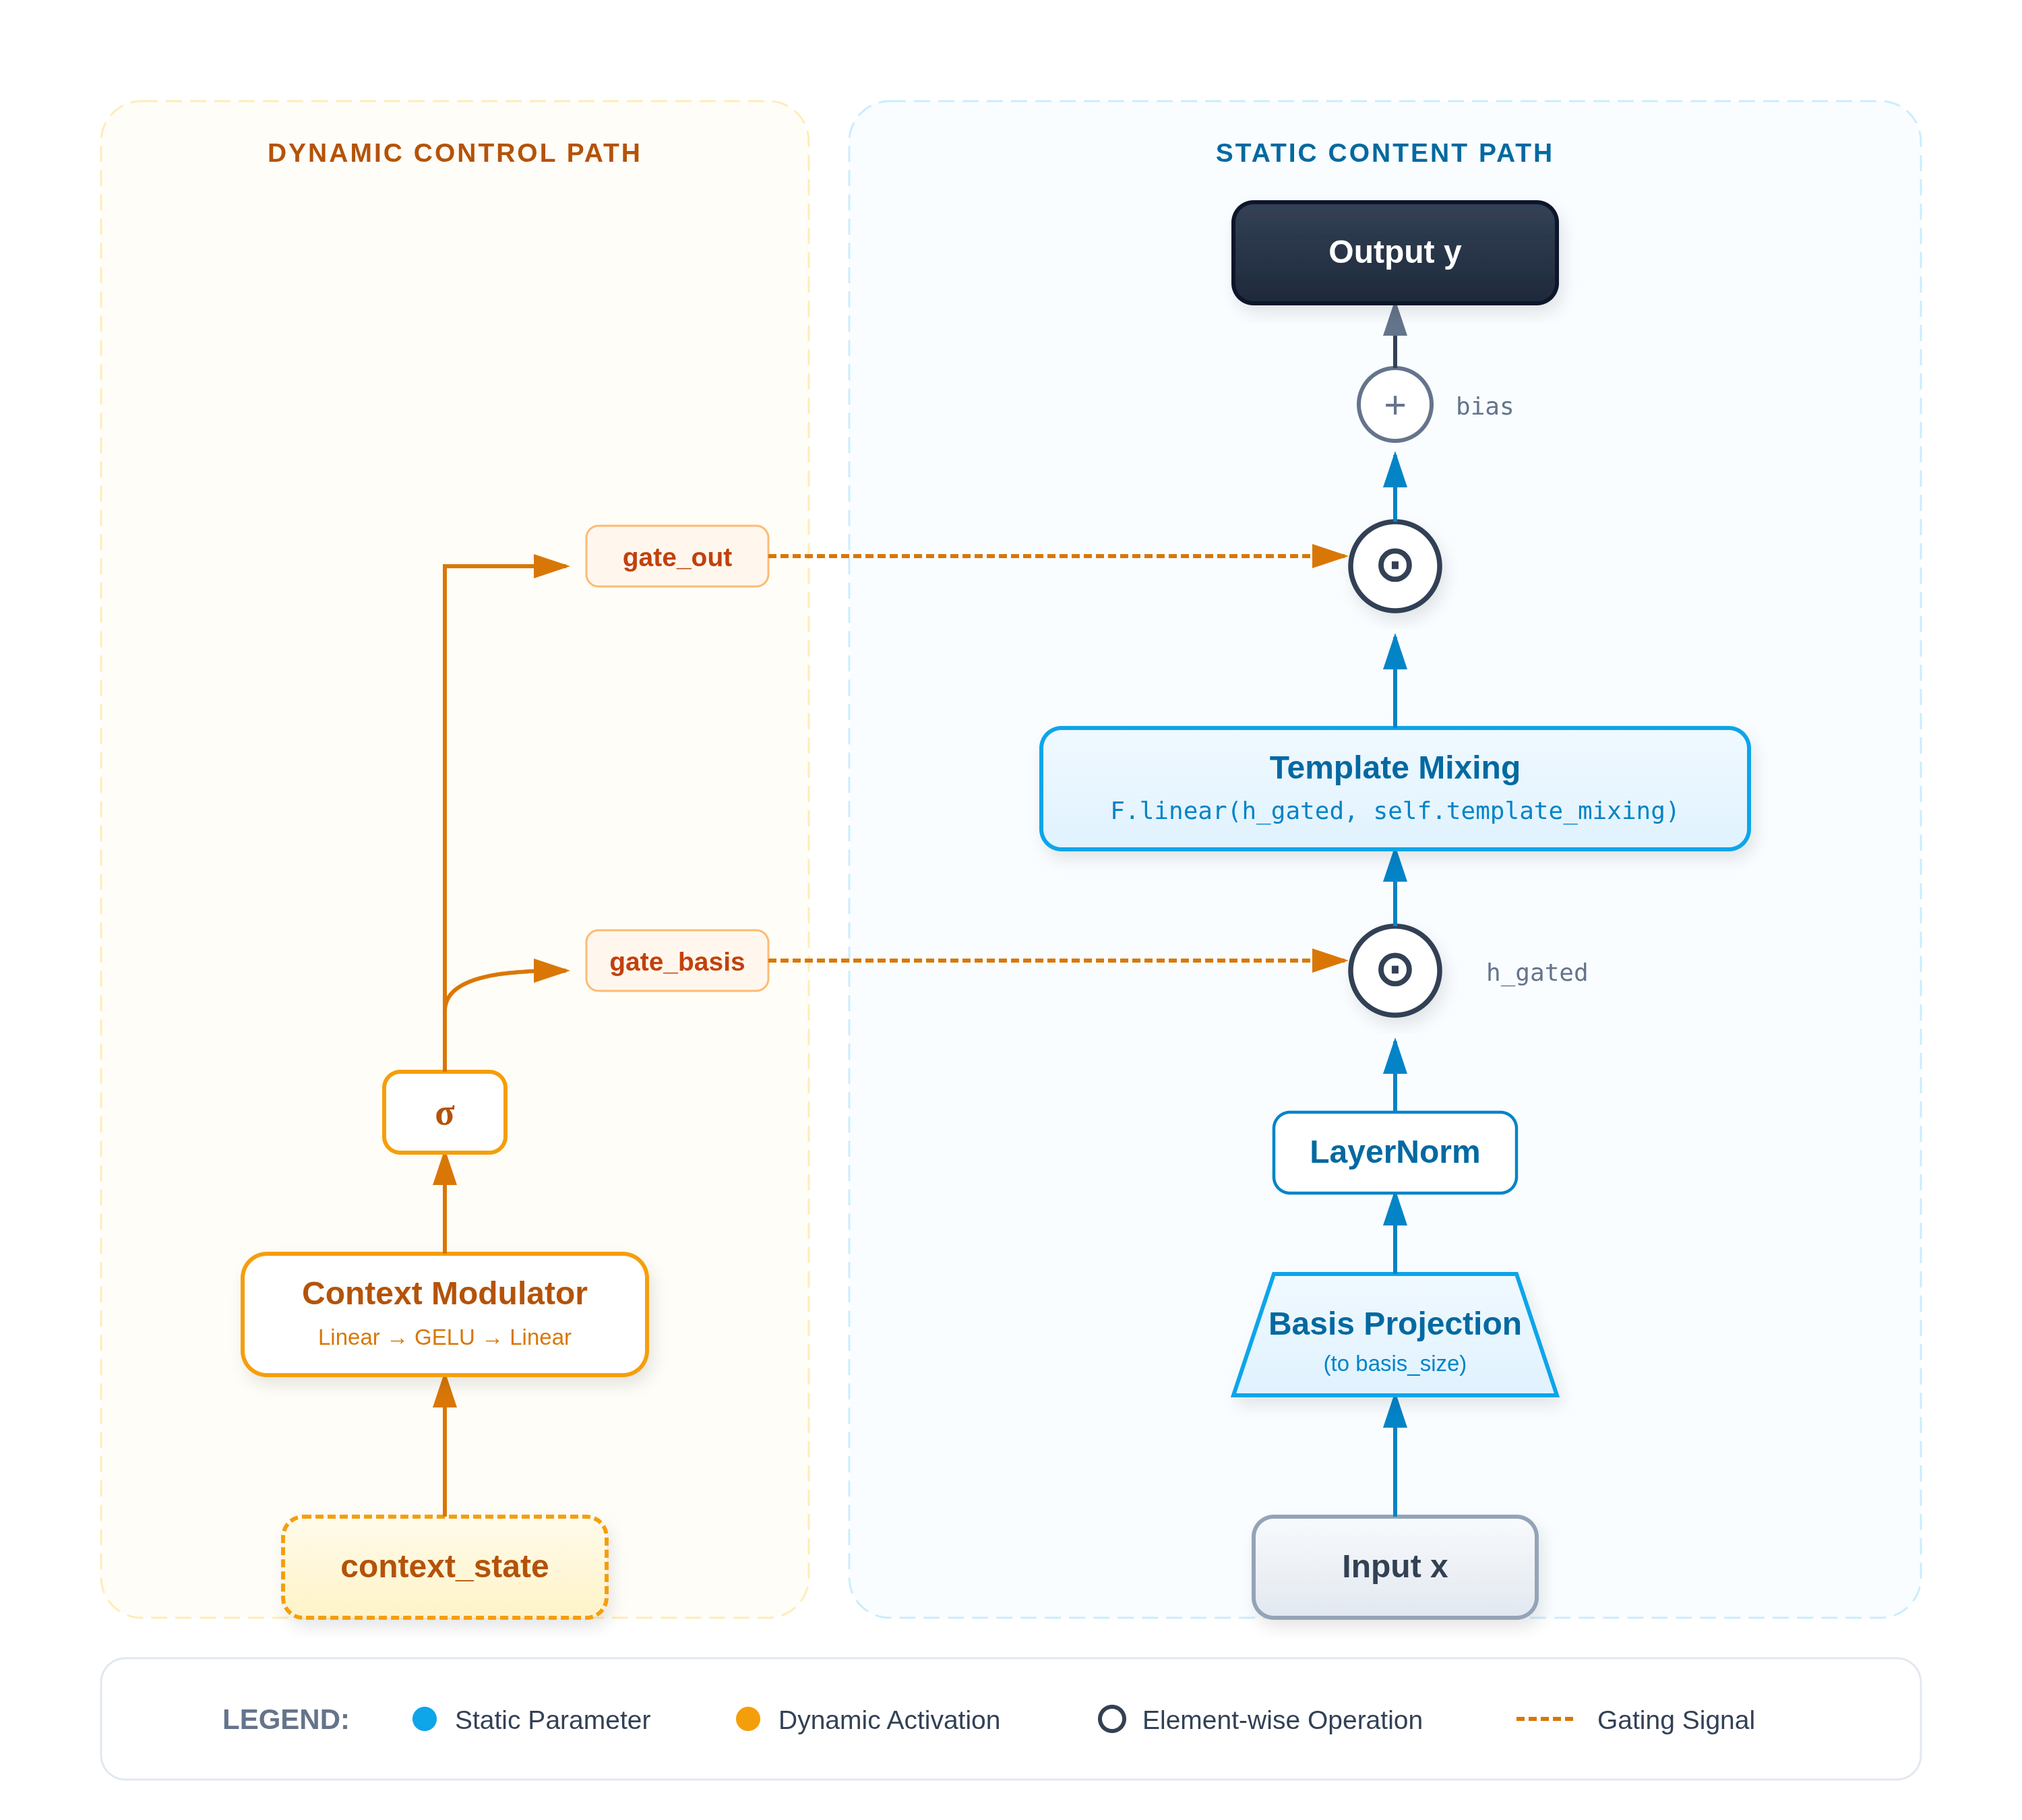
\includegraphics[width=0.7\textwidth]{ccll_architecture.png}
\caption{Architecture Overview of the Context-Conditioned Linear Layer (CCL). A shared context signal modulates all linear layers without sparse routing. }
\label{fig:architecture}
\end{figure*}
% \vspace{1em}

\begin{figure*}[!htbp]
% \vspace{1em}
% \begin{figure}[H]
\centering
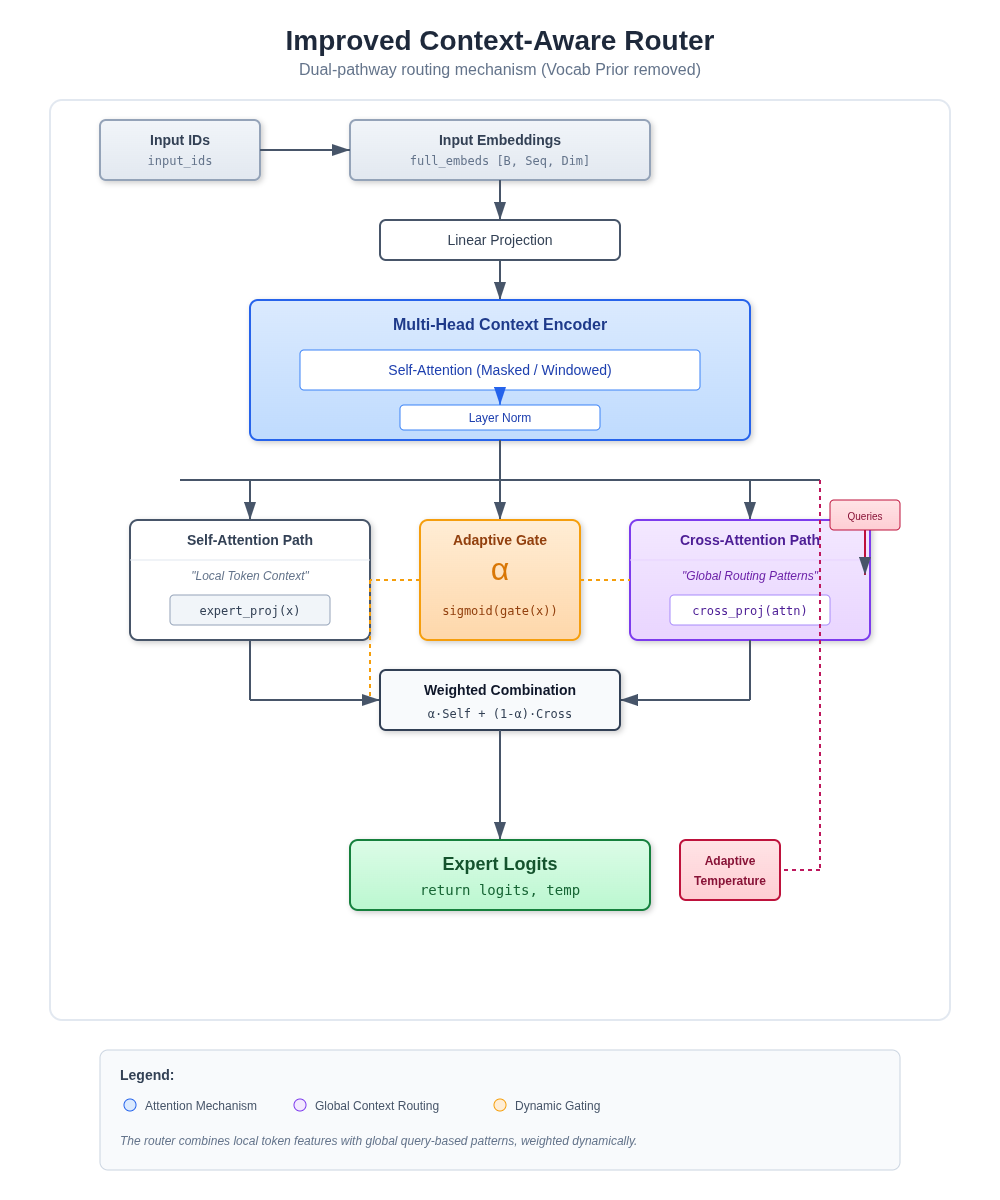
\includegraphics[width=0.5\textwidth]{context_aware_router.png}
\caption{Global Context Manager}
\label{fig:router_architecture}
\end{figure*}
\section{Method}
\begin{figure}[t]
\begin{minipage}{\columnwidth}
\small
\begin{verbatim}
class CCL(nn.Module):
  def __init__(self, d_in, d_out, d_ctx, k=64):
    self.basis = Linear(d_in, k, bias=False)
    self.mix   = Parameter(d_out, k)
    self.gate  = MLP(d_ctx, k + d_out)
    self.bias  = Parameter(d_out)
    self.norm  = LayerNorm(k)

  def forward(self, x, c):
    h = self.norm(self.basis(x))      # basis projection
    g = sigmoid(self.gate(c))         # context gates
    g_b, g_o = split(g)               # basis / output gates
    h = h * g_b
    y = linear(h, self.mix)           # static mixing
    return y * g_o + self.bias
\end{verbatim}
\end{minipage}
\caption{Simplified implementation of the Context-Conditioned Linear layer.
Context modulates only low-dimensional gating vectors, while all matrix
multiplications remain static and dense.}
\label{fig:remixedlinear}
\end{figure}

We introduce the \textbf{Context-Conditioned Linear Layer (CCL)}, a drop-in replacement for the standard dense linear layers found in Transformer Feed-Forward Networks (FFNs).

\subsection{Standard vs. Context-Conditioned Formulation}
A standard linear layer computes $y = xW + b$, where $W \in \mathbb{R}^{d_{in} \times d_{out}}$ is a static parameter matrix. This forces $W$ to capture a compromise of all possible semantic transformations required by the model.

In CCL, we replace $W$ with a dynamic composition of a static \textit{Basis Dictionary}. For an input token representation $x \in \mathbb{R}^{d_{in}}$, the computation proceeds in three stages:

\paragraph{1. Basis Projection.}
We project the input into a latent basis space using a static matrix $W_{basis} \in \mathbb{R}^{d_{in} \times d_{basis}}$, where $d_{basis}$ is a hyperparameter (typically $d_{basis} \ll d_{in}$).
\begin{equation}
    h_{basis} = \text{LayerNorm}(x W_{basis})
\end{equation}
Normalization is applied to ensure stable signal propagation before modulation.

\paragraph{2. Context-Aware Modulation.}
A lightweight \textbf{Global Context Manager} $\mathcal{C}$ computes a context vector $c_t$ for the token. A modulator network $\phi$ then generates a gating vector $g_{basis} \in [0, 1]^{d_{basis}}$:
\begin{equation}
    g_{basis} = \sigma(\phi(c_t))
\end{equation}
where $\sigma$ is the sigmoid function. This gate dynamically selects active basis features (ingredients) relevant to the current semantic context. The modulated representation is computed via element-wise multiplication:
\begin{equation}
    \tilde{h} = h_{basis} \odot g_{basis}
\end{equation}

\paragraph{3. Template Mixing and Output.}
The modulated basis features are mapped to the output dimension via a static template matrix $W_{mix} \in \mathbb{R}^{d_{basis} \times d_{out}}$. To further refine the output, a second gate $g_{out} \in [0, 1]^{d_{out}}$ (generated by $\phi$) filters the activations:
\begin{equation}
    y = (\tilde{h} W_{mix} + b) \odot g_{out}
\end{equation}

\subsection{Expressed Capacity Analysis}
Although the operation involves low-rank matrices ($d_{basis} < d_{in}$), the effective linear operator $W_{eff}^{(t)}$ applied to token $t$ is:
\begin{equation}
    W_{eff}^{(t)} = W_{basis} \cdot \text{diag}(g_{basis}^{(t)}) \cdot W_{mix} \cdot \text{diag}(g_{out}^{(t)})
\end{equation}
Since the gating vectors $g^{(t)}$ vary for every token, $W_{eff}^{(t)}$ changes dynamically. While any single $W_{eff}^{(t)}$ is rank-constrained by $d_{basis}$, the union of operators $\{W_{eff}^{(1)}, \dots, W_{eff}^{(T)}\}$ across a sequence spans a high-dimensional subspace. This allows CCL to exhibit high \textit{expressed capacity} without the memory cost of storing a full-rank matrix.

\subsection{Complexity}
The parameter cost of CCL is dominated by $W_{basis}$ and $W_{mix}$, totaling roughly $d_{in} \times d_{basis} + d_{basis} \times d_{out}$. For $d_{basis} \ll d_{in}$, this yields significant compression. The computational overhead is limited to the generation of gate vectors ($O(d)$), maintaining the hardware efficiency of dense matrix multiplication.

\subsection{Relation to Low-Rank and Expert Models}

CCL can be viewed as a generalization of low-rank linear layers. A static low-rank projection restricts all inputs to a fixed subspace defined by $\mathbf{W}_{\text{basis}}$ and $\mathbf{W}_{\text{mix}}$. In contrast, CCL modulates both basis activations and output mixing as a function of context, producing token-specific effective weight matrices.

Unlike mixture-of-experts models, CCL does not route tokens to discrete experts or rely on sparse execution. Instead, all tokens share the same parameters while inducing different linear transformations via continuous gating. This avoids gather–scatter operations and preserves efficient dense execution on modern accelerators.

\subsection{Effective Rank Perspective}

Although each effective transformation is low-rank, the set of transformations realized across a sequence varies with context. As a result, the induced operators span a substantially higher-dimensional space than static low-rank layers. We empirically validate this property via effective-rank analysis in Section~\ref{sec:experiments}.

\section{Experiments}
\label{sec:experiments}
\subsection{Experimental Setup}
We evaluate Context-Conditioned Linear Layers (CCL) by replacing the feed-forward linear projections in a standard Transformer language model. All models are trained from scratch on the same corpus with identical optimization settings. Model quality is measured using validation perplexity (PPL). Computational efficiency is evaluated using dense FLOPs per token and throughput (tokens/sec), measured at batch size 64 and sequence length 64.
All models are trained from scratch with identical token budgets, the AdamW optimizer, and a OneCycle learning rate schedule over 5,000 steps. We observe that CCL models are more stable and performant at moderately higher learning rates.
\begin{table*}[t]
\centering
\caption{Perplexity results across all methods. The \textbf{CCL (64-dim)} approach outperforms all baselines, including the 512-dim Dense Baseline, despite using 8x fewer dimensions. \textbf{Bold} indicates best performance.}
\label{tab:combined_results}
\resizebox{\textwidth}{!}{
\begin{tabular}{lcccccc}
\toprule
\textbf{Model} & \textbf{Active Dim} & \textbf{WikiText-103} & \textbf{Penn TreeBank} & \textbf{Text8} & \textbf{Enwik8} & \textbf{LAMBADA} \\
\midrule
\multicolumn{7}{l}{\textit{Dense Baselines}} \\
\quad Baseline (512-dim) & 512 & 92.35 & 50.11 & 187.83 & 54.66 & 189.20 \\
\quad Baseline (64-dim) & 64 & 238.30 & 57.64 & 448.13 & 111.07 & 301.47 \\
\midrule
\multicolumn{7}{l}{\textit{Ours: Context-Conditioned Linear Layer}} \\
\quad \textbf{CCL(64-dim)} & \textbf{64} & \textbf{55.83} & \textbf{26.47} & \textbf{150.49} & \textbf{49.65} & \textbf{70.88} \\
\bottomrule
\end{tabular}
}
\end{table*}


\subsection{Baselines}
We compare against dense Transformer baselines with hidden sizes $\{64, 256, 512\}$, trained under identical settings. We additionally report results for selection-based and remixing-style variants where applicable. These baselines isolate the effects of static width scaling, expert selection, and dynamic basis composition.

\subsection{Efficiency and Performance}
Table~\ref{tab:efficiency} reports parameter counts, FLOPs per token, and inference throughput. CCL models achieve substantially better efficiency–performance trade-offs than dense baselines. In particular, \textbf{CCL-64} matches or outperforms larger dense models while operating at similar FLOPs per token as Base-64, demonstrating that context-conditioned linear operators provide additional expressive capacity beyond static width scaling.
\begin{table}[t]
\centering
\caption{Efficiency analysis. Comparison of parameter count, dense FLOPs per token, and throughput in tokens per second under full-sequence parallel inference (batch size 64, sequence length 64). FLOPs are estimated via THOP and represent dense execution upper bounds.}

\label{tab:efficiency}
\small
\resizebox{\columnwidth}{!}{
\begin{tabular}{@{}lcccc@{}}
\toprule
\textbf{Model} & \textbf{Params} & \textbf{FLOPs/token} & \textbf{Tokens/sec} \\
 &  & (MFLOPs) &  \\
\midrule
Base-512 & 44.70M & 89 & 70,644 \\
Base-256 & 30.54M & 35 & 161,831 \\
Base-64  & 6.79M   & 7  & 523,081 \\
\midrule
\textbf{CCL-64} & \textbf{10.29M} & \textbf{7} & \textbf{364,155} \\
\bottomrule
\end{tabular}
}
\end{table}


\begin{figure}[t]
    \centering
    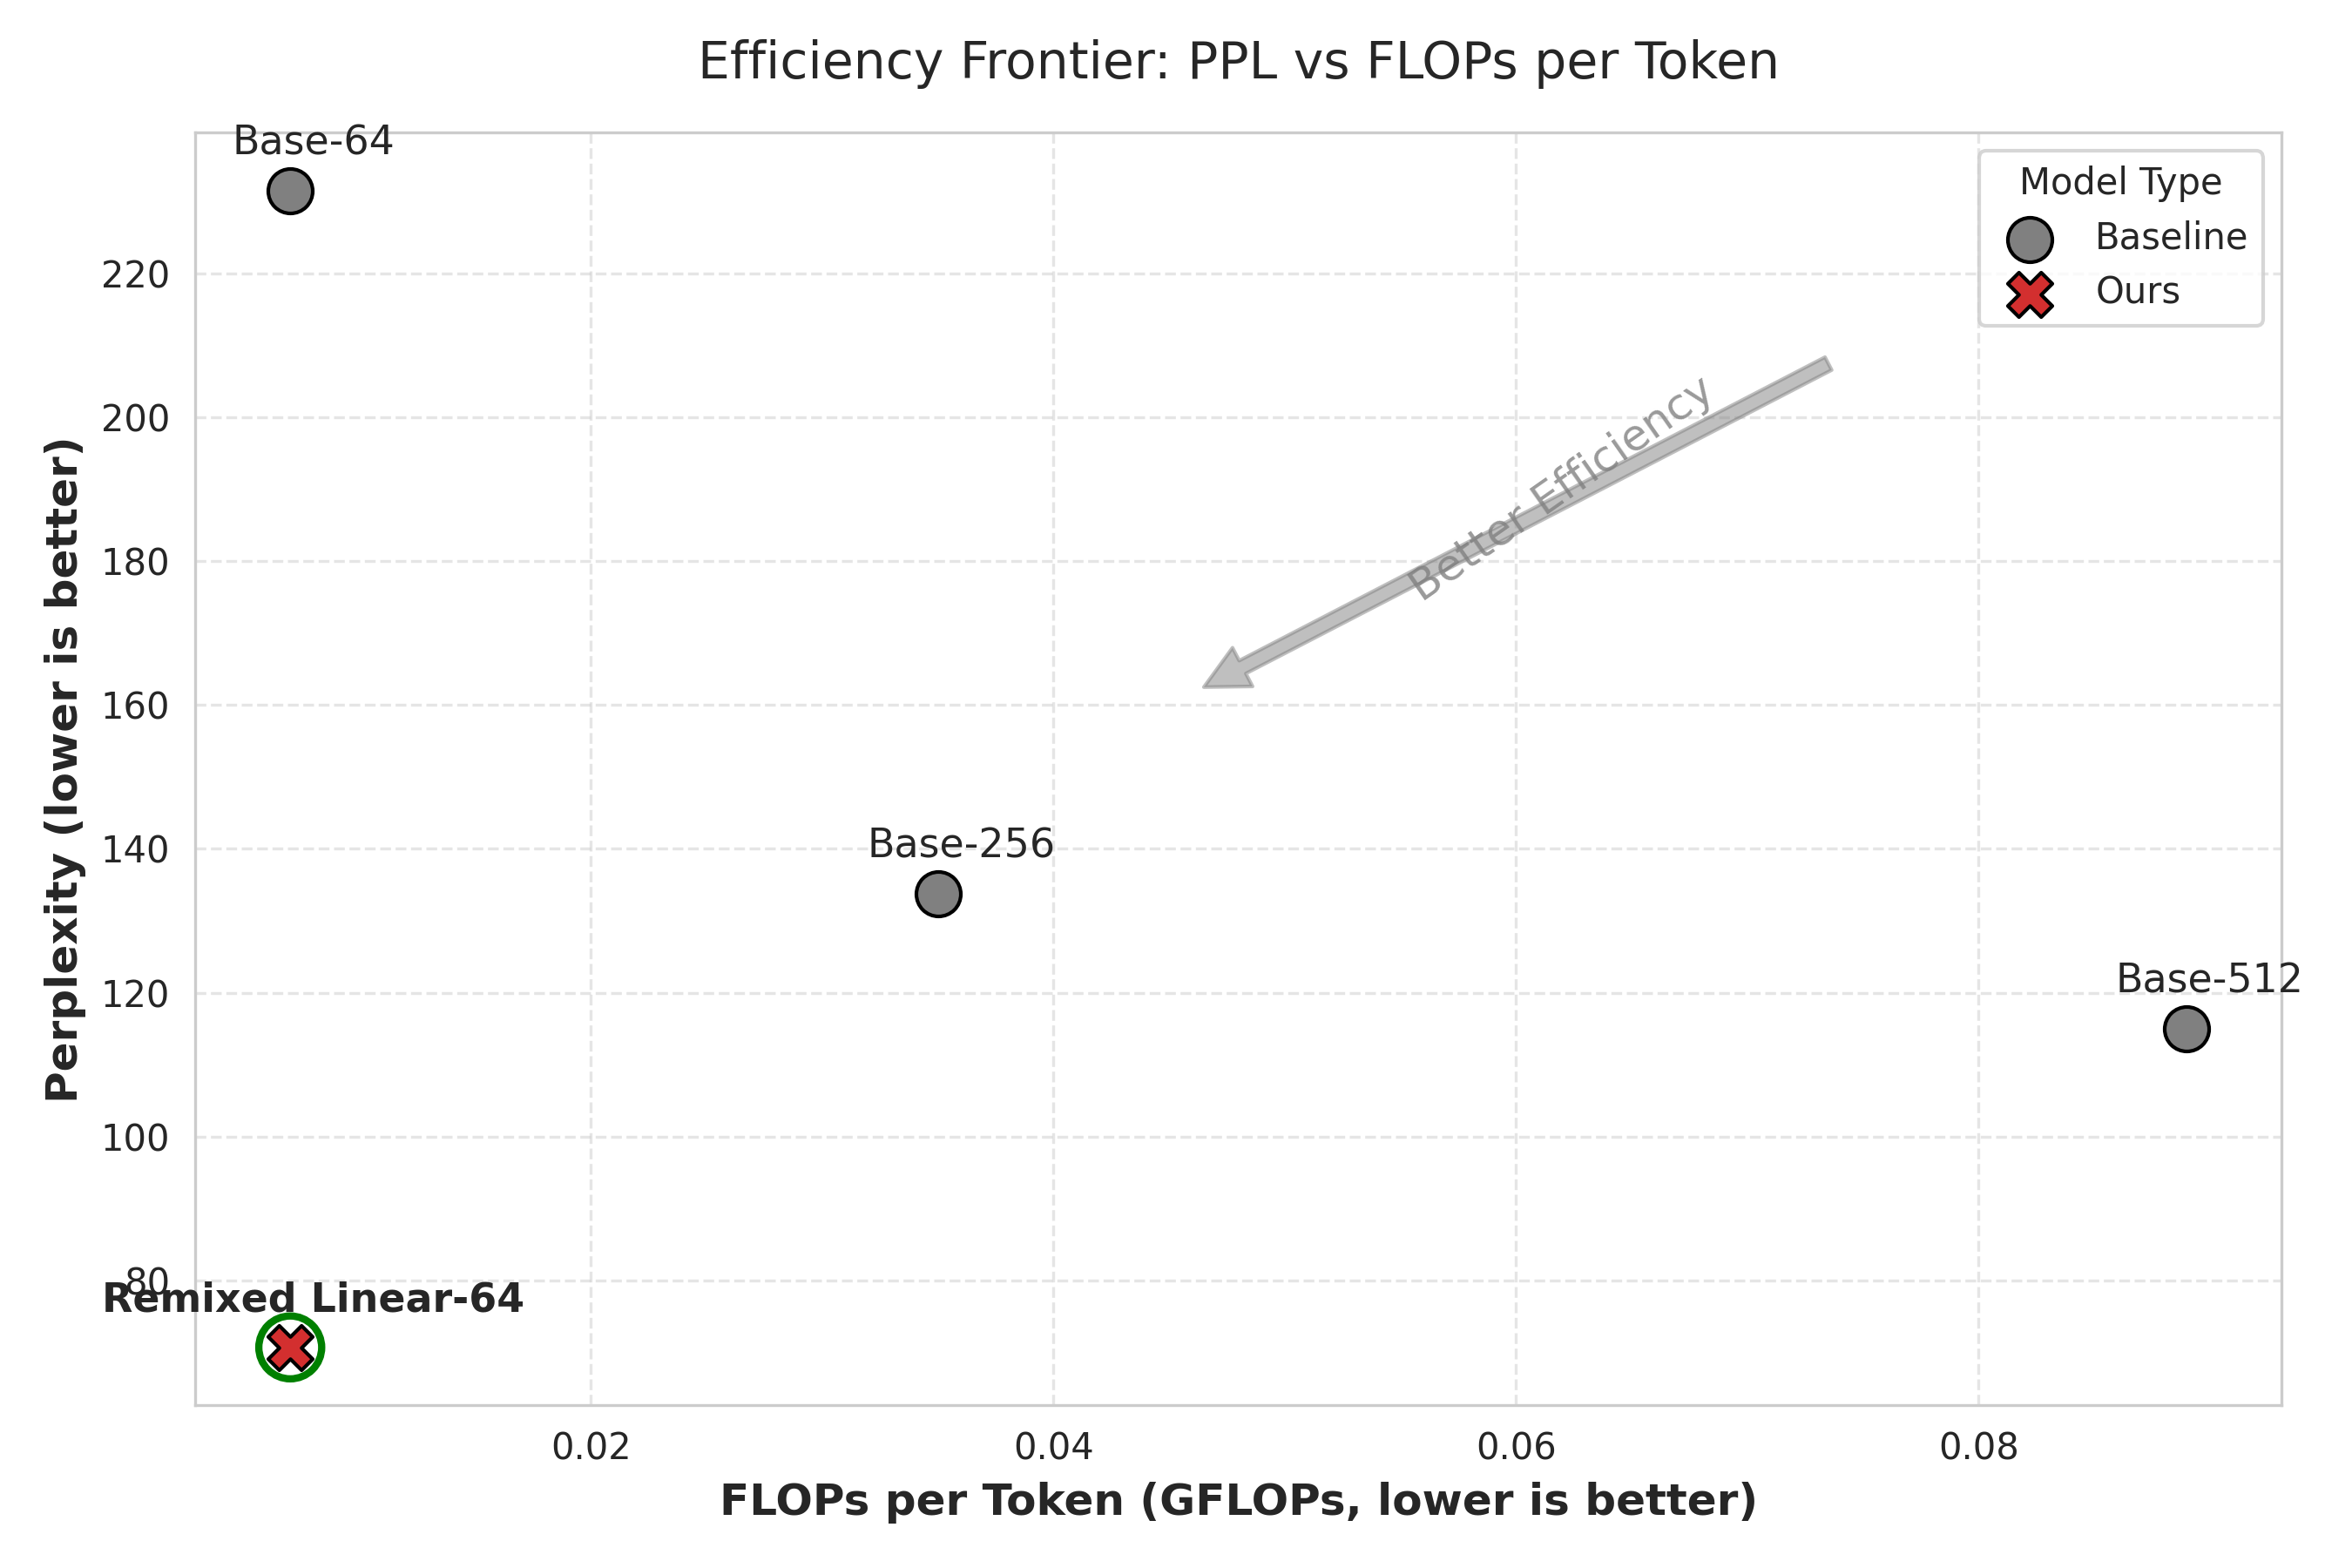
\includegraphics[width=0.9\columnwidth]{ppl_vs_flops_frontier.png}
    \caption{Perplexity vs.\ FLOPs per token. Lower is better on both axes. The arrow indicates the direction of improving efficiency. CCL models occupy a more favorable region of the Pareto frontier than dense baselines.}
    \label{fig:ppl_flops}
\end{figure}

Figure~\ref{fig:ppl_flops} visualizes this effect. While dense models follow a predictable trade-off between FLOPs and perplexity, CCL shifts the frontier, achieving lower perplexity at comparable or lower computational cost.
 As shown in Table \ref{tab:combined_results}, the CCL architecture achieves lower perplexity across all datasets.

We achieve a \textbf{38\% reduction in perplexity} while using \textbf{6.8X fewer parameters} than the standard high-capacity baseline. Furthermore, as shown in Table \ref{tab:combined_results}, CCL maintains the FLOPs profile of a much smaller model (Base-64), confirming that the dynamic gating mechanism introduces negligible computational overhead ($<0.1\%$ increase in FLOPs).
\subsection{Effective Rank Analysis}
To understand the source of these gains, we analyze the effective rank of the induced linear operators. Although each token-level operator is low-rank, the collection of operators across a sequence exhibits a slow singular value decay, indicating a high-dimensional span.

\begin{figure}[t]
    \centering
    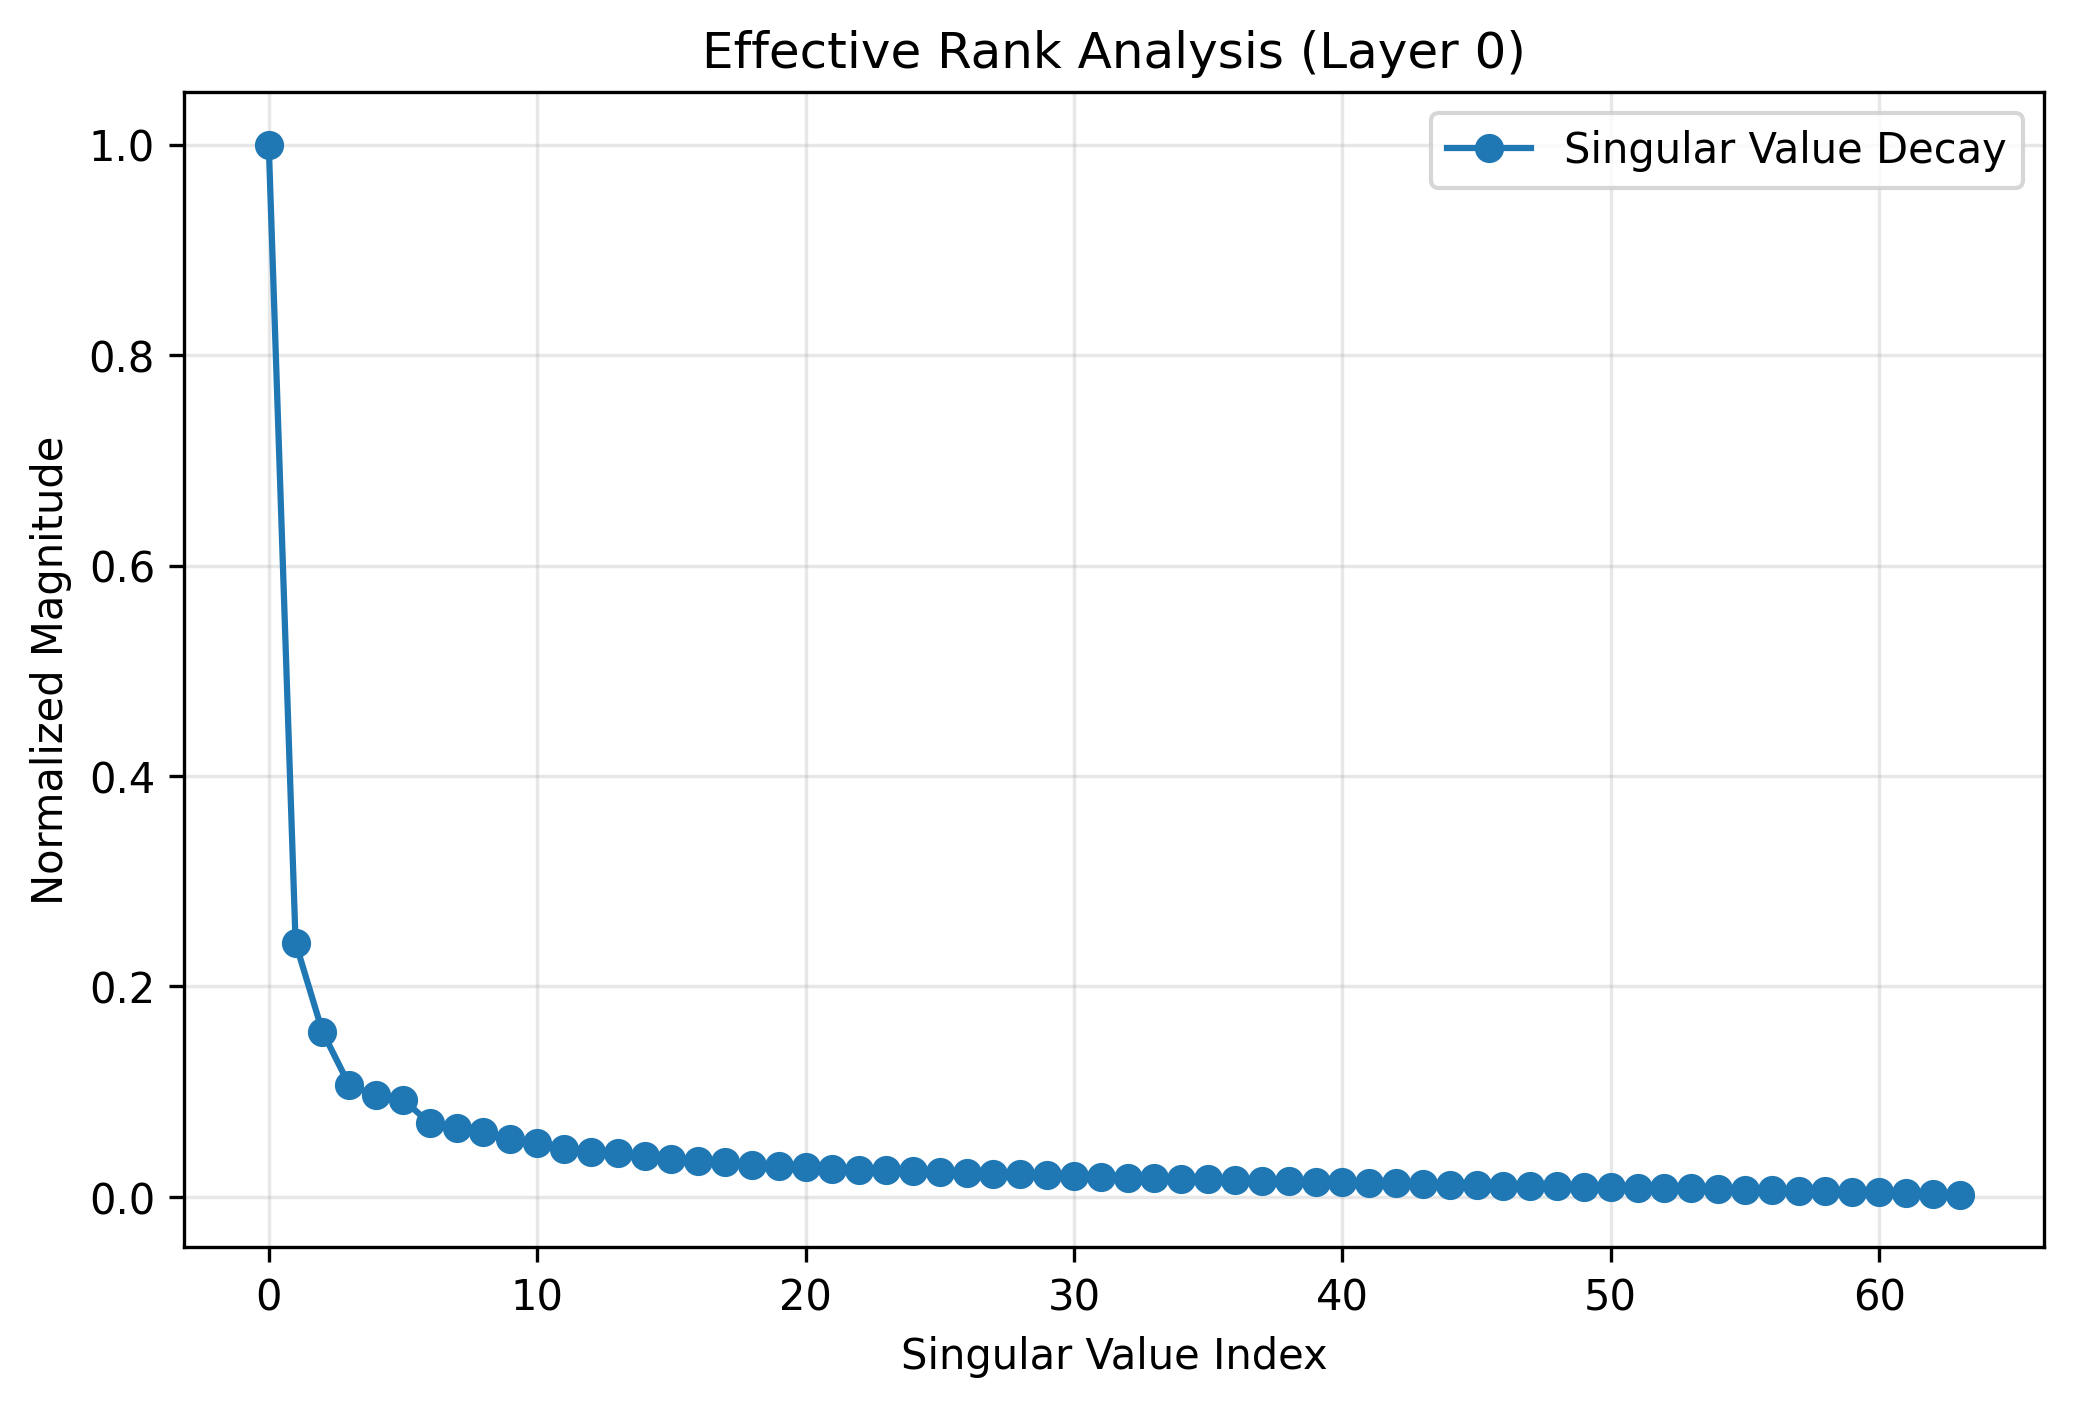
\includegraphics[width=0.9\columnwidth]{effective_rank.png}
    \caption{Singular value decay of effective linear operators across a sequence. The slow decay indicates high expressed rank despite low-rank parameterization.}
    \label{fig:effective_rank}
\end{figure}
Figure \ref{fig:effective_rank} reveals a ``long tail'' in the singular value spectrum. While the first few components capture core syntax, the spectrum remains active well beyond the rank of the static basis. This confirms our hypothesis: the \textbf{expressed capacity} of the model—the manifold spanned by its operators across time—is significantly higher than its \textbf{stored capacity}.

This confirms that CCL overcomes the expressivity bottleneck of static low-rank layers by varying the active subspace with context.



\subsection{Gate Utilization}
We further analyze gate behavior to assess utilization and specialization. Gates exhibit balanced activity, with the majority operating in a mid-range regime rather than saturating. Basis gates consistently activate for semantically related tokens, indicating reusable lexical and semantic components.
We investigate whether the model learns static scaling or actively switches modes. We analyze the distribution of gate activation values on the validation set. Figure \ref{fig:gate_hist} visualizes the distribution of gate activation. 
\begin{itemize}
    \item \textbf{Bimodal Distribution:} The gate values follow a U-shaped distribution (Entropy $\approx 0.43$), with peaks near 0 and 1. This indicates the Context Manager learns a discrete-like routing strategy, making ``hard'' decisions to fully activate or suppress features.
    \item \textbf{Active Modulation:} Over 55\% of gates fall in the active decision range, refuting the notion that the gates simply saturate or collapse to a static mean.
\end{itemize}


\begin{figure}[t]
    \centering
    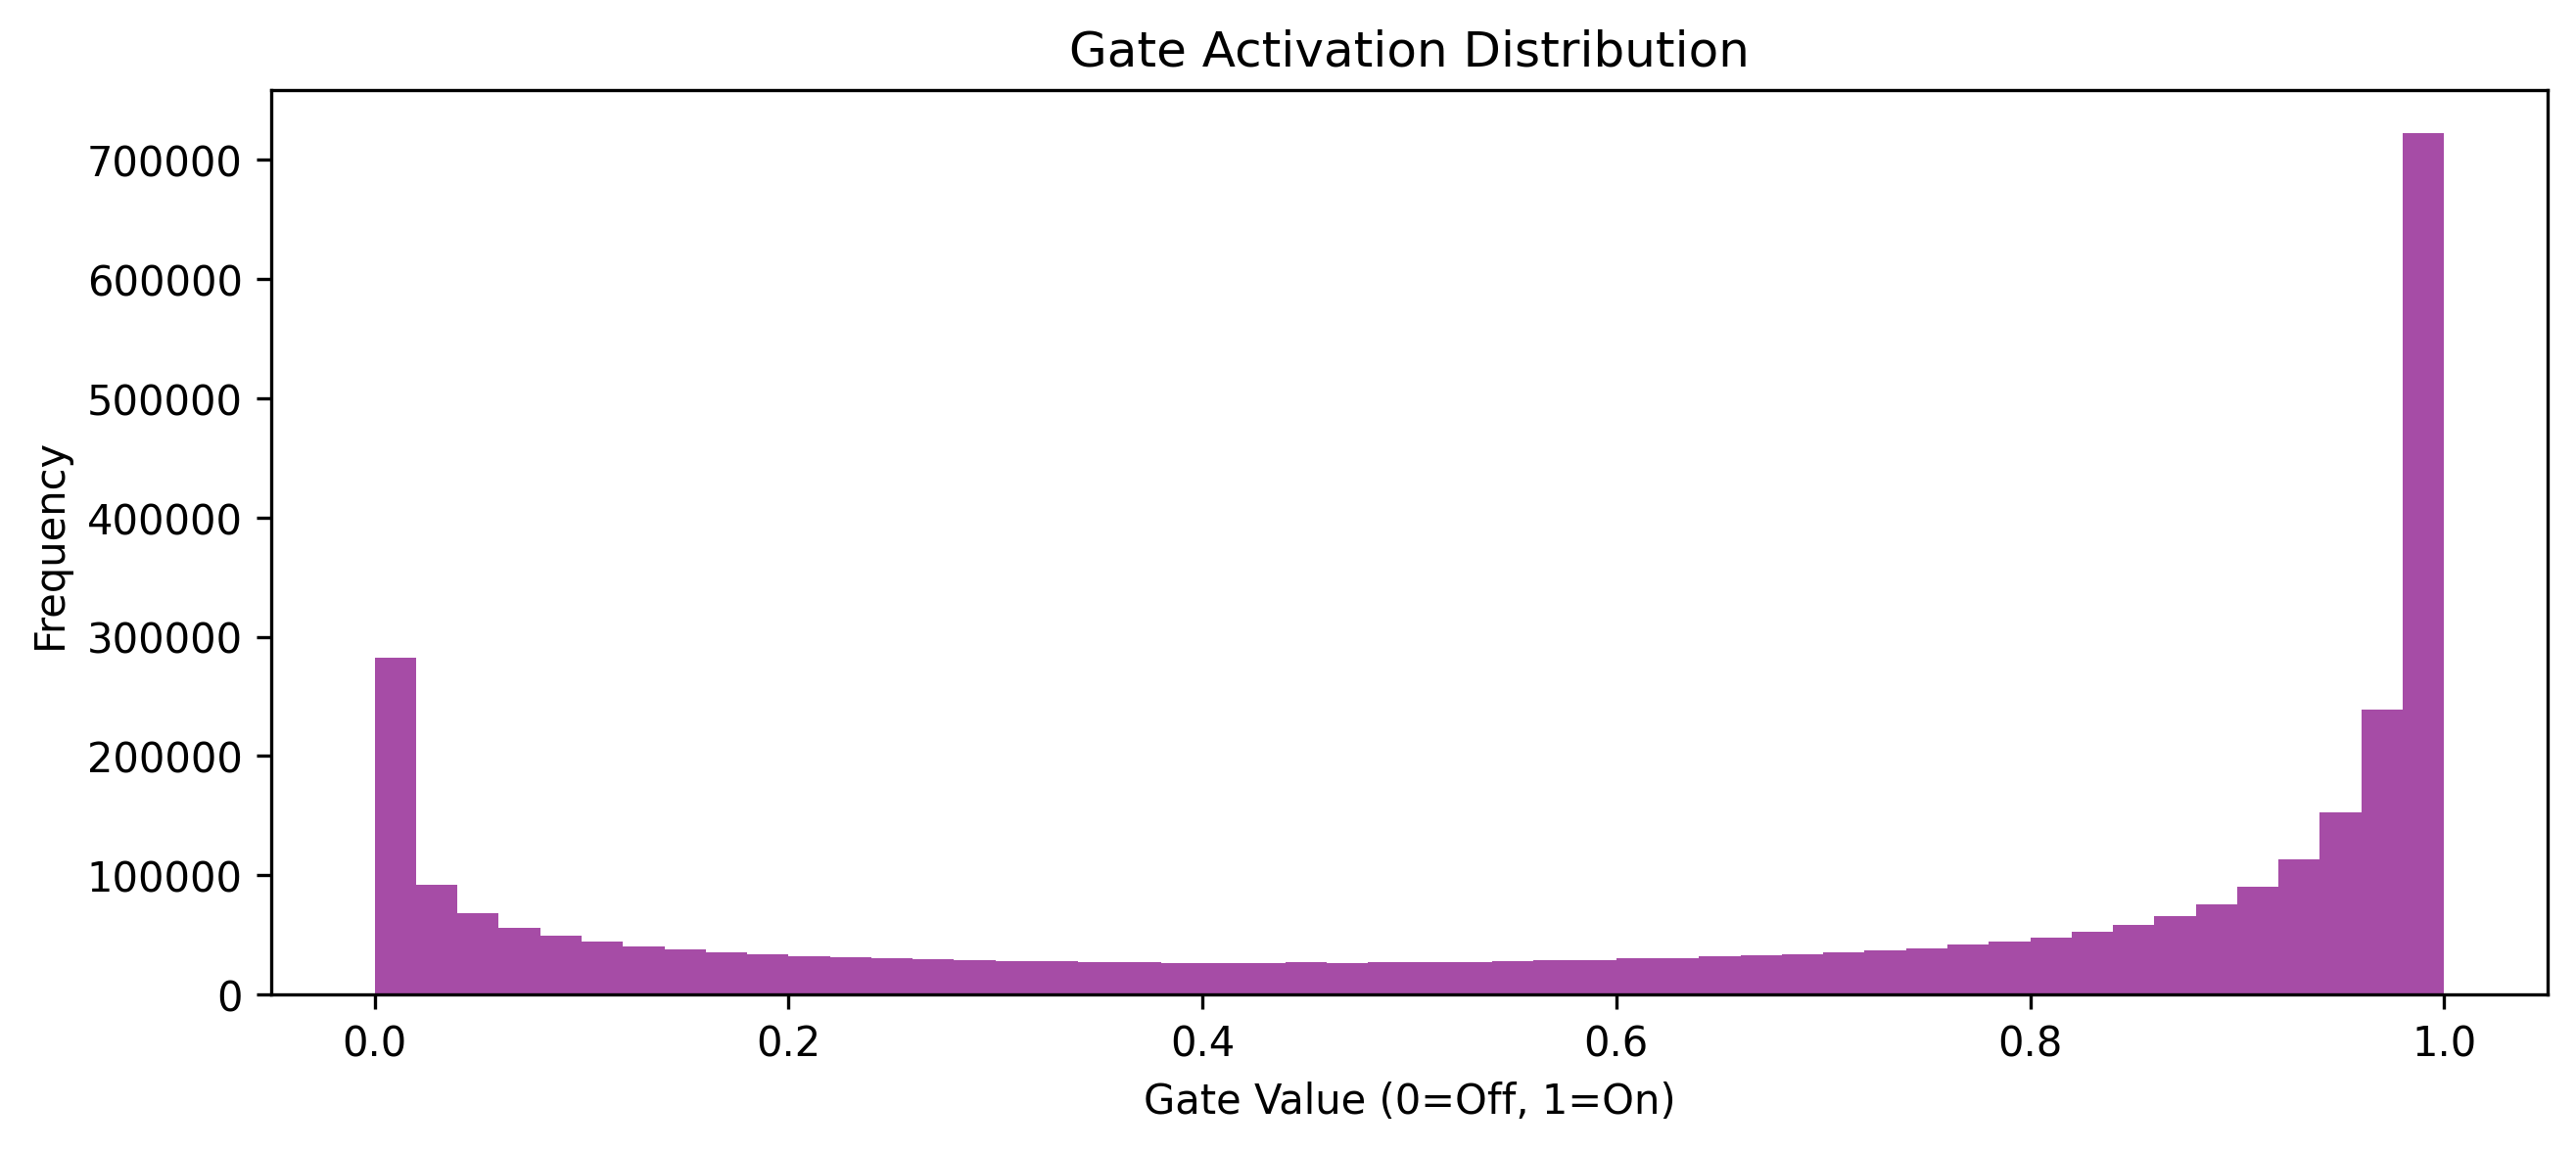
\includegraphics[width=0.9\columnwidth]{gate_statistics.png}
    \caption{Distribution of gate activations. Most gates operate in an active, non-saturated regime.}
    \label{fig:gate_hist}
\end{figure}

\begin{figure}[t]
    \centering
    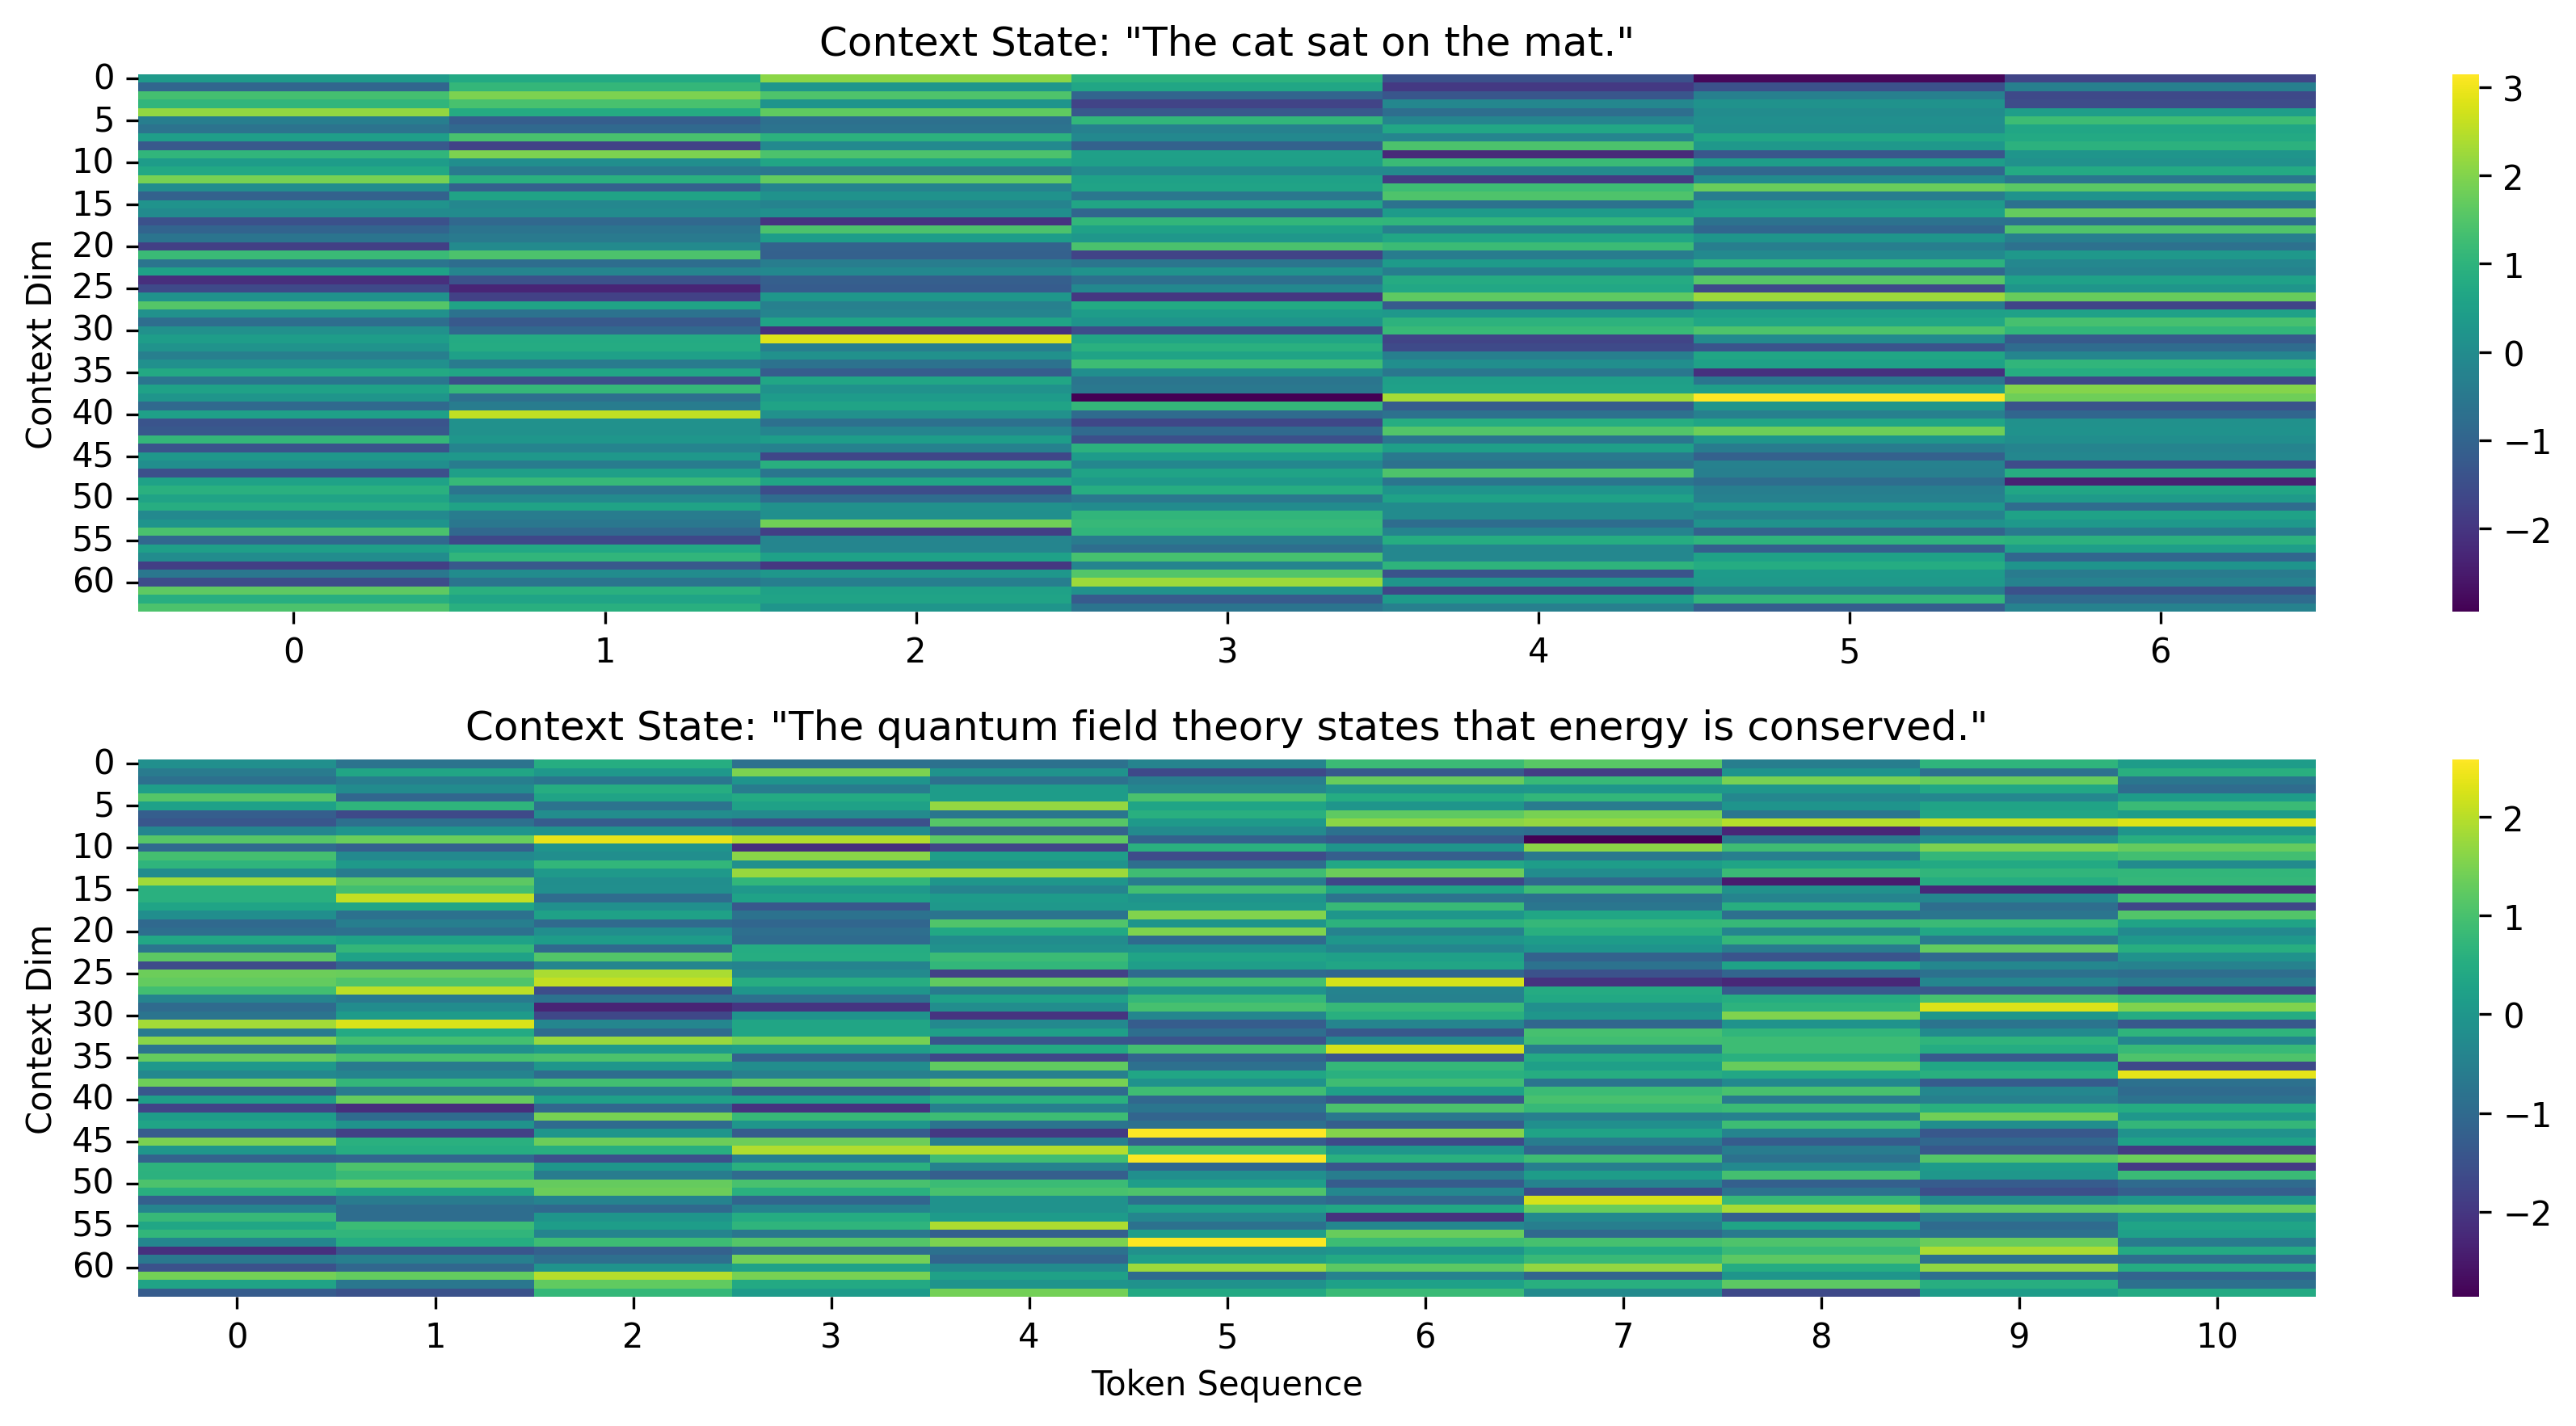
\includegraphics[width=0.9\columnwidth]{context_fingerprint.png}
    \caption{Context fingerprints for different input sequences, illustrating token-dependent modulation of linear operators.}
    \label{fig:context_fingerprint}
\end{figure}

Together, these analyses indicate that CCL increases \emph{expressed capacity} without increasing \emph{stored capacity}. By preserving dense execution and avoiding sparse routing, CCL translates theoretical FLOPs reductions into practical throughput gains.

\subsection{Gate Specialization and Interpretability}

To assess whether basis gates learn meaningful functional roles rather than acting as uniform scaling factors, we analyze the tokens that most strongly activate individual gates. Table~\ref{tab:gate_specialization} shows the top-ranked tokens routed to selected basis gates.

Each gate exhibits clear semantic coherence. For example, Gate~3 primarily activates on past-tense verbs, Gate~4 captures proper nouns and institutional entities, and Gate~7 responds to adjectival and demonym-like terms. This indicates that gates specialize in reusable semantic or lexical functions rather than encoding token identity.

Importantly, this specialization emerges without discrete routing or expert partitioning. All tokens share the same parameters, while continuous gating induces soft, interpretable subspaces. This supports the view that CCL increases expressed capacity by context-dependent operator selection, rather than by duplicating parameters.
This interpretability suggests that CCL disentangles linguistic factors into discrete basis vectors, which are then recomposed as needed.

\begin{table}[t]
\centering
\small % Optional: Makes font slightly smaller to fit tight spaces
\caption{Top tokens routed to selected Basis Gates, showing learned specialization patterns. The middle column wraps to prevent overflow.}
\label{tab:gate_specialization}
\begin{tabularx}{\linewidth}{@{} c X c @{}}
\toprule
\textbf{Expert} & \textbf{Top Tokens} & \textbf{Specialization} \\
\midrule
Gate 3 & gained, instructed, performed, raised, transported & 1.00 \\
Gate 4 & mates, performed, Oregon, Wright, university & 1.00 \\
Gate 7 & real, American, Ol', Willow, Australian & 1.00 \\
\bottomrule
\end{tabularx}
\end{table}


\subsection{Ablation Study}
To verify that these gains stem from dynamic context conditioning rather than architectural artifacts, we perform an ablation study (Table \ref{tab:ablation}).
\begin{itemize}
    \item \textbf{Static Baseline:} Removing the Global Context Manager (setting gates to identity) causes performance to degrade sharply (PPL 151.39). This confirms that the low-rank basis alone is insufficient; the \textit{dynamic modulation} is the primary driver of performance.
    \item \textbf{Gate Contribution:} Removing the output modulation ($g_{out}$) degrades performance to 63.54, while removing basis gates degrades it to 69.99, demonstrating that filtering activations is as critical as selecting features.
\end{itemize}

\begin{table}[h]
    \centering
    \caption{Ablation of dynamic components. ``Static'' removes context conditioning entirely. Lower perplexity is better.}
    \begin{tabular}{lc}
        \toprule
        \textbf{Configuration} & \textbf{Perplexity} \\
        \midrule
        Static Linear (No Context) & 151.39 \\
        No Output Gate & 63.54 \\
        No Basis Gate & 69.99 \\
        \textbf{Full CCL} & \textbf{59.19} \\
        \bottomrule
    \end{tabular}
    \label{tab:ablation}
\end{table}

\section{Discussion}

\paragraph{Dynamic Capacity without Sparsity.}
The central trade-off in modern Transformer design has been between the hardware efficiency of dense layers and the scaling potential of sparse MoE models. CCL resolves this by introducing a new category of layer: the \textit{dynamic dense} layer. By retaining a dense computational graph, CCL avoids the memory fragmentation and communication overheads associated with token routing in MoE \cite{fedus2022switch}. Our throughput results confirm this: despite the additional logic of the Context Manager, CCL achieves real-world latency comparable to standard dense layers, translating theoretical FLOPs reductions into actual speedups.

\paragraph{Beyond Static Low-Rank Adaptation.}
While techniques like LoRA \cite{hu2021lora} have popularized low-rank factorization for adaptation, they remain static during inference. Our Effective Rank analysis demonstrates why this is insufficient for pre-training: a static bottleneck permanently limits the model's expressivity. CCL demonstrates that the \textit{rank} of a layer need not be a static property of its geometry but can be a dynamic property of its forward pass. This suggests that future architectures should optimize for \textit{expressed capacity} (the manifold of operators) rather than \textit{stored capacity} (parameter count).

\section{Conclusion}

We introduced Context-Conditioned Linear Layers (CCL), a simple drop-in replacement for dense linear projections that dynamically constructs token-specific linear operators from a compact shared basis. By conditioning linear transformations on context, CCL decouples \emph{expressed capacity} from \emph{stored parameters}, overcoming the expressivity limitations of static low-rank layers without relying on sparse expert routing.

Empirical results show that CCL achieves strong perplexity improvements under matched parameter and FLOPs budgets, while effective-rank and gate-specialization analyses confirm that the model realizes a diverse set of meaningful transformations across a sequence. Importantly, CCL preserves hardware-efficient dense execution, allowing theoretical efficiency gains to translate directly into practical throughput improvements.

These findings suggest that context-conditioned linear operators provide a promising alternative to both static compression methods and mixture-of-experts architectures for building efficient Transformer models.


\section{Limitations} \label{sec:limitations} While our results demonstrate the efficacy of context-conditioned linear layers, we acknowledge several limitations. \textbf{Scale:} Our experiments were conducted on models up to 70M parameters due to compute constraints. While the efficiency gains are promising, verifying whether these trends hold for large-scale foundation models (e.g., 7B+ parameters) remains future work. However, since CCL is fundamentally a drop-in replacement for linear layers, we see no architectural barriers to scaling. Although our method improves batched throughput, the Global Context Manager introduces a fixed computational cost per step. For extremely latency-sensitive, single-stream applications (batch size of 1), this routing overhead might offset the gains from reduced embedding dimensionality.
CCL introduces a new hyperparameter: the basis size $d_{basis}$. While we found $d_{basis}=64$ to be robust across our experiments, optimal performance likely requires scaling $d_{basis}$ relative to the model width $d_{model}$, necessitating further study into optimal scaling ratios.

\section*{Acknowledgements}
In accordance with the AI Writing Assistance Policy, we acknowledge the use of large language models (specifically Gemini,Claude, and ChatGPT) to assist with rephrasing text for clarity, condensing sections to meet page limits, and refining mathematical notation. All generated text was reviewed, verified, and edited by the human authors, who take full responsibility for the content.
\bibliography{references}  % Your .bib file

\end{document}


% This document was modified from the file originally made available by
% Pat Langley and Andrea Danyluk for ICML-2K. This version was created
% by Iain Murray in 2018. It was modified from a version from Dan Roy in
% 2017, which was based on a version from Lise Getoor and Tobias
% Scheffer, which was slightly modified from the 2010 version by
% Thorsten Joachims & Johannes Fuernkranz, slightly modified from the
% 2009 version by Kiri Wagstaff and Sam Roweis's 2008 version, which is
% slightly modified from Prasad Tadepalli's 2007 version which is a
% lightly changed version of the previous year's version by Andrew
% Moore, which was in turn edited from those of Kristian Kersting and
% Codrina Lauth. Alex Smola contributed to the algorithmic style files.
